\documentclass[a4paper,11pt]{report}
\title{DeepDepth \\ An Approach To Visualize Twitter Tweets}
\author{AmirSaber Sharifi}
\date{October 2014}
\pagestyle{headings}

\usepackage{listings}
\usepackage{color}
\usepackage{ifthen}
\usepackage{hyperref}


\setcounter{tocdepth}{3}
\setcounter{secnumdepth}{3}

\definecolor{dkgreen}{rgb}{0,0.6,0}
\definecolor{gray}{rgb}{0.5,0.5,0.5}
\definecolor{mauve}{rgb}{0.58,0,0.82}

\lstset{frame=tb,
  language=Java,
  aboveskip=3mm,
  belowskip=3mm,
  showstringspaces=false,
  columns=flexible,
  basicstyle={\small\ttfamily},
  numbers=none,
  numberstyle=\tiny\color{gray},
  keywordstyle=\color{blue},
  commentstyle=\color{dkgreen},
  stringstyle=\color{mauve},
  breaklines=true,
  breakatwhitespace=true
  tabsize=3
}

\usepackage{graphicx}
\graphicspath{ {./images/} }

\newboolean{includeMemo}
\setboolean{includeMemo}{true} % boolvar=true or false

\newcommand{\memo}[1]{
  \ifthenelse {\boolean{includeMemo}}{\medskip\noindent\fbox{\begin{minipage}[b]{\dimexpr\linewidth-1em}#1\end{minipage}}\medskip\newline}
}

\begin{document}

\maketitle

\tableofcontents

\listoffigures

\chapter{Introduction}

\section{Social Networks}

A \emph{social network} is a “structure of relationships linking \emph{social actors}” or “the set of actors and the ties among them”\cite{stankath}. Relationships or ties are the basic building blocks of human experience, mapping the connections that individuals have to one another \cite{pescosolido}\cite{socialnetworkdef}. Social Networks are typically defined as a social structure made up of a set of social actors, who can be individuals or organizations, and a set of \emph{dyadic ties} between these actors. Being friends, relatives or colleges are examples of possible dyadic ties.

As the world becomes more interconnected through the \emph{World Wide Web}, social networks are becoming more relevant through World Wide Web. When these relations happen through World Wide Web they are called \emph{Social Web}. In general, Social Web is a set of relationships that link people over the World Wide Web\cite{socialwebw3}. Social Web covers the design and develop of software or web pages that encourage social interactions using Word Wide Web. Examples of some Social Web implementation can be games, education and social networking websites. Facebook, Google Plus, Tumbler and Twitter can be named as examples of social networking websites.

Depend on the social networking website, social actors can be individuals, organizations and groups and social dyadic ties between these actors also depends on the social networking website. As an example in Twitter, both individuals and organizations can have accounts and they can interact with other actors by following others, posting a message, replying to other actor messages and re-post a message that has been originally posted by other actor.

These social networking websites can get benefits to individuals and organizations. As an individual, making friends, chatting, posting photos and having social interactions in general can be expected as a benefit of a social networking website. Creating online communities so users with common interests can join and socialized around the topic or find old school friends on these websites are some other benefits of social web for individuals.

On the other hand organization can use social networking websites to reach their audiences easier. They can establish communities and pages to reach more audiences and even use smart advertisement tools to advertise their message to specific group of people. By looking at trends and hit rate of their posts they can make better decisions for their future activities or products. These are some examples of benefits for organizations while a lot more can be imagined using social network websites and related analytic tools designed for them.

Each social network could be analyzed with different perspectives. One can be analyzing social network structures to identify patterns and examine network dynamics. The other can be analyzing social network data. These data can be the message that a user posts or a color they choose as background or even time of the day users are active on social networks.

Twitter is one of the famous social networking website. Users in Twitter can read and post 140 character short messages that are called \emph{tweets}. Twitter provide various ways of posting a tweet like using their web site, application or text messages. It's established on March 2006 and since then it grows fast between users\cite{twitterstat}. There are about 284 million active users on Twitter. Users on Twitter post average of 6,000 tweets per second which correspond to 350,000 tweets per minute and 500 million tweets per day\cite{twittercompany}. Twitter also supports more than 35 languages. This is a substantial amount of data that can be used in different analyses.

Twitter provides a substantial amount of information of each tweet. Information like user number of tweets, user profile color, language and etc. These information can be useful also. One example can be looking at relation between profile color of users and their tweets about committing suicides. By implementing an appropriate tool one can analyze Twitter tweets, or any other social networking websites, in different perspectives and get useful and meaningful results. For instance by watching and monitoring tweets which contains symptoms of a disease over time, origin of a disease could be found or even prevent the next possible epidemic.

\section{DeepDepth}

Our goal in this master project is to design a modular platform called DeepDepth to provide an infrastructure for analyzing and visualizing social network data. DeepDepth is able to connect to specific sources of social network data and then be configured to define various analyzes and their required visualizations.

Administrator is able to exapand and manage DeepDepth which means an administrator with knowledge of programming can add query types, graphs or even new social network source into the platform. In the first iteration of the platform, Twitter is considered as the main source of data, although other sources can be added to project later.

Since DeepDepth is a social network related service users are able to login using their social network identity or create their own username. DeepDepth will help them to access visualized meaningful social network data without having vast knowledge of computer science. They are able to tweek results to their need. Since using social network websites is growing, various entities such as researchers, laboratories and industries found social network websites a good resource of information. Noticing the importance of social network websites on our life and benefits that a good analytic tool could give us, idea of DeepDepth shaped.

\section{Related works}

Here are some other similar systems available on web that do analytic on social network data. Some of those systems are as follow:

\paragraph{Orgnet.com SNA}
Social Network Analysis (SNA) is a tool that does mapping and measuring of relationships and flows between actors. It provides mathematical and visual analysis of social network and calculate different degrees for each node such as betweenness and closeness.\cite{orgnet}

\paragraph{Twazzup} A monitoring tool to show users each time their keyword is mentioned in a tweet.\cite{twazzup}

\paragraph{Twitscoop} was a real-time visualization tool that could tank tweet words based on how frequently they are used.\cite{twitscoop}

\paragraph{TweetPsych} is a web application that uses linguistic analysis algorithms to create a profile for a person based on what they have been tweeted on Twitter.\cite{tweetpsych}

\paragraph{Tweeps} analyzes the content of user's tweets and make statistic for that specific user. This service is currently down.\cite{tweeps}

\paragraph{Twitonomy} analyzes activity of a user in twitter. It can gives some general numbers like average number of tweets per day or users most mentioned and active hours and days. \cite{twitonomy}

Most twitter Monitoring and Analytics tool are not working any more because of Twitter change in their API policy which doesn't let third party apps to have access to all tweets using their API. Companies which want to have access to all tweets should go into a contract with Twitter\cite{twitterfirehose}.

DeapDepth is different from these examples in essence that DeepDepth is more general. It's a platform that administrator of it can add graphs, query types and etc so users will be able to use different kinds of analytic and visualizations. It's more dynamic that means DeepDepth can also get connected to different data sources and do analyzes on them. These data sources can be Facebook, Google+ or any other social network in future.

\section{Challenges}

To implement DeepDepth there were some challenges. This challenges happened in different aspect of project. For instance in gathering data, storing data, processing data and visualizing the result.

The first step in analyzing a data is the data and gather it. Since DeepDepth is a modular application, it can use any Hive database as it source of analyzes. For Twitter scenario gathering data has been done by using Twitter Official client for developers which is called HBC. It's a client for a stream API that receive a sample of all tweets. Since HBC should be an always running process it's running in a PaaS named Heroku\cite{herokuadd}. Heroku is also the service that help storing the data using its Treasure Data\cite{treasuredataadd} api.

Processing data was a challenge that could be handled in various ways. One can suggest using Apache Storm\cite{apachestormadd} which results in a real time analysis. Because of required resources to do real time processing, DeepDepth is using an on demand processing. MapReduce is the technique that is used to process a Hive database entries.

After the process phase results need to be visualized. To be able to have a modular application a framework of drawing charts and graphs should be considered so administrator and developers can later add graphs to the project easily. So in DeepDepth Visualizing data part is implemented using D3.JS\cite{d3jsadd} library which is a graph framework that is able to draw specific charts and graphs and also can be programmed to draw custom graphs and charts. By using D3.Js a lot of ready to use charts are available to use in DeepDepth and developer or administrator can also add other graph types to it.

\chapter{DeepDepth}

\memo{
\begin{itemize}
\item Implementation of server and client sides using Test Driven Development
\end{itemize}
}

\section{High-Level Description}

\subsection{Components}

\memo{WY: How about combining Chapters 2 and 3 and call it DeepDepth. Then, you have a section called "High-Level Description", which is your Section 2.1 now, and then you have another section called "Implementation Details" which has the subsections on Server and Client. Then, within these subsections, you briefly describe the technology that you use, why you chose to use it, and how you use it. 

\begin{itemize}
\item What are the programmer work space and environment provided for this project.
\item What are the components in this project and briefly describe them
\item How those components are related and how they interact
\item Work flow Diagram
\item Data flow Diagram
\item Use Cases, what are user types and how different users see the project and how they use this software
\end{itemize}
}

\subsubsection{Major Components}

DeepDepth has been made out of 4 major components. Social data collector, Social data database, Web Application and Web application database. All of these components are programmed in a cloud IDE, C9, and are available to access their code via gitHub. Figure \ref{fig:majorcomponents} shows how DeepDepth major components are connected and how they interact with social networks.

\begin{figure}[!ht]
\begin{center}
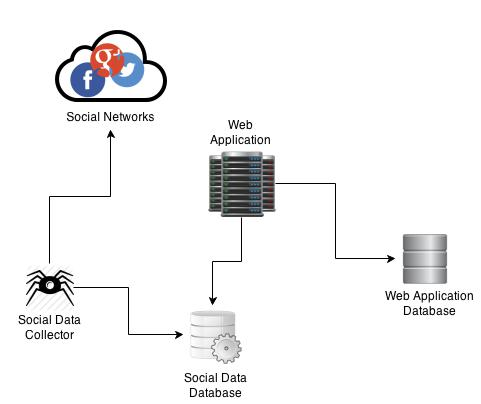
\includegraphics[scale=0.5]{majorcomponents.jpg}
\end{center}
\caption{How major components are connected}
\label{fig:majorcomponents}
\end{figure}

Social data collector is the application that is responsible of collecting data from social networks and store them into social data database. This can be done in various ways. It can be done by connecting to social network APIs, crawling their web site, getting streams and etc. At the same time Social data collector should saved the retrieved data into a database. Social data collector is an on going application that should be always working and gather as much as data possible into database.

Social data database is the destination of Social data collector for saving data. Since social data is a big data, the database should be capable of storing bulk data and should also be able to run large, complex queries in an acceptable time. For this reason a database with MapReduce capablities is a well fitted database.

After receiving and storing data into database, Web application component should enable the platform for users to access the data and run their own queries against the Social data database. Web application is the component that users directly interact with using web protocols. To maintain different types of users, status of requested queries and etc Web application needs to access to a database to store it's data.

Web application database doesn't need to ba a bulk database neccesserly. Since the main process is going to happen on Social data database, Web application database is only for general information of the application such as user names, password, query types and etc.

\subsubsection{Web Appication}

Web application is the main component in DeepDepth. Web application is the component that connects Social data database to users and provide the required interface for users to submit their queries into database and get their results back.

Users are able to register into application by accessing the Web application via internet and then sign up there. Sign up process can be done by using existing user services such as Google and Facebook, or by creating a local user in Web application. Figure \ref{fig:usersregister} show how the register process works.

\begin{figure}[!ht]
\begin{center}
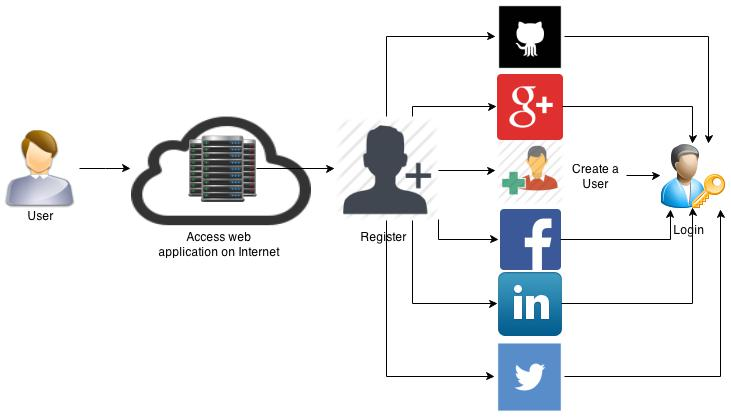
\includegraphics[scale=0.5]{users_register.jpg}
\end{center}
\caption{Register process}
\label{fig:usersregister}
\end{figure}


Web application consider two types of roles, admins and users. Admins are the users who have permission to do the required configuration for data sources and query types. Then users can login and select from the defined query types and data sources and generate their queries based on their need and submit it to database to get results. Figure \ref{fig:userslogin} demonstrate that after the user authenticate itself into system their role is assigned to them based on database information.

\begin{figure}[!ht]
\begin{center}
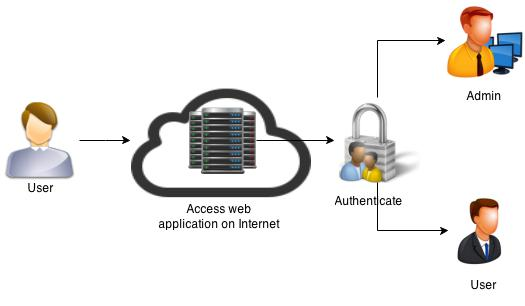
\includegraphics[scale=0.5]{Users_login.jpg}
\end{center}
\caption{Login process}
\label{fig:userslogin}
\end{figure}

After logging into Web application based on the user role, Web application provide different functionalities for them. An admin is able to create Field types, Graph types and Job types. Each query should have a Job type that defines the type of the query, the required fields to run the query and the graphs that can be drawn for that query. When a user choose a Job type, Web application would fetch the required Field types and ask the user to fill them to be able to run the query.

The main responisibility of admin is to create and maintain Job types. Job types are created of Graph types, Field types, Query pattern and source. Source means the database address that the query should be sent to. Field types are the required fields that are needed to run the query with. Query pattern is the pattern that will genertate the final query based on what user puts into fields and the Graph types are the graphs that can be drawn based on the chosen Job type. Figure \ref{fig:datarelation} shows the raltion of data between entities.

\begin{figure}[!ht]
\begin{center}
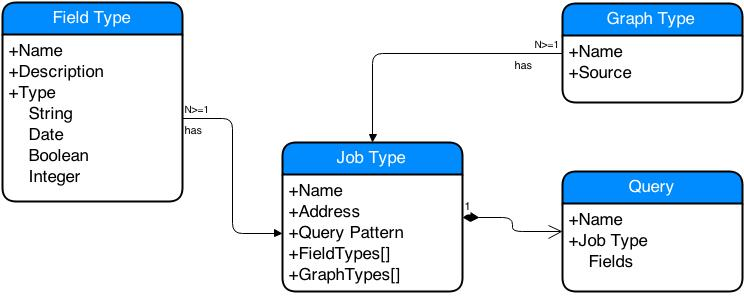
\includegraphics[scale=0.5]{datarelation.jpg}
\end{center}
\caption{Field type, Graph type, Job type and Query relation}
\label{fig:datarelation}
\end{figure}

When an admin logs into DeepDepth, Field types should be defined. After defining Field types, Graph types should be defined. Using Field types and Graph types, Job types could be defiend and users are able to use it. Figure \ref{fig:adminuse} shows the use case of admin.

\begin{figure}[!ht]
\begin{center}
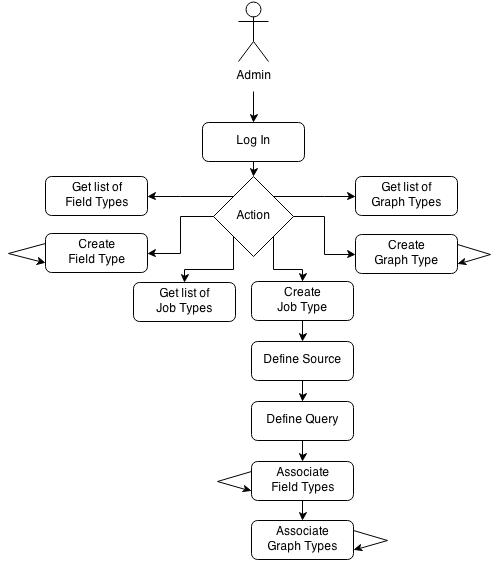
\includegraphics[scale=0.5]{adminuse.jpg}
\end{center}
\caption{Admin use case}
\label{fig:adminuse}
\end{figure}

\subsection{Technologies}

\memo{
\begin{itemize}
\item Describe the technology that have been used in this project for each component
\item More detail into each component and how they interact with each other
\end{itemize}
}

\subsubsection{Social data}

A Social data collector can be written in various ways. In initial version of DeepDepth it's uses a Java application which connects to Twitter Filter endpoint to recieve tweets from Twitter which are filtered based on their location. The chosen location is mainland of United States. Since it connects to Filter endpoint it will recieve a sample of tweets which are about 1\% of all tweets in U.S. To be able to have all tweets it needs to connect to Firehose endpoint of Twitter which is not free for use. Since this application needs to be an always running application and connected application, it's running in Heroku PaaS.

For each tweet that the Social data collector recieve from Twitter stream it needs to save it to database. DeepDepth is using Treasure Data service to stores it's data. Treasure Data is a company which provides Hive databases as service. Treasure data can also be used as a plug in into Heroku application. So Social data collector is able to store its recieved tweet into a Hive database using Treasure Data service.

Hive is a database that can be queried using a SQL like language named HiveQL. These queries will be queued and then executed as MapReduce jobs in Hive. Query execution time varies based on the query and the number of processors associated to Treasure Data account. In the initial version of DeepDepth only one processor is being used.

\subsubsection{Web Application}

Web application component of DeepDepth is implemented using MEAN stack. MEAN stack contains, MongoDB as database, Express.JS as it's web server, Angular.JS for it's browser side and Node.JS as the programming language.

On the server side, Node.JS has been used which is a javascript based platform. It's hosting Express.JS web framework for web and http requests. Grunt.JS is used for task automation during building process and debugging process. For the Web application to be able to recover from crashes, Forever.JS has been used. Since DeepDepth is developed in a Test Driven Environment, Should.JS and Phantom.JS are used for testing porposes. JSHint is also used to make sure of clean Javascript code. In the build process by using CSSHint and Uglify.JS, a compact version of required Javascripts and CSS files are created for the client side.

On the client side, DeepDepth is using Single Page Application model. Angular.JS is used to achieve SPA. Jquery is the other Javascript library used in client side for manipulating and controlling HTML elements. D3.JS is used to implement and draw graphs and charts. For User Interface elements of Web application, Bootstrap is being used. For templating purposes of application Jade is being used.

For local data that are needed by Web application, such as Usernames, Queries, Job Types and etc. DeepDepth is using MongoDB which is a document oriented database. On DeepDepth there is a RESTful implementation of Web API's so other future applications would be able to use it as a service. To implement the RESTful API on top of the database, Mongoose has been used.

\section{Implementation}

\subsection{Server}

\memo{
\begin{itemize}
\item What is the server side and what it is doing
\item How components in server side have been implemented
\end{itemize}
}

DeepDepth Web Application server side has been made of 4 major components. These 4 components are App, Config, Node Modules and Public. App is the main component that works on the server side and is reponsible of recieving requests and replying to request using RESTFul APIs. Config is the component that is responsible for required configuration such as port numbers and then initialize the application with them. Node Modules is the component that consist of other Node.JS ready to use components. Public is what a user will get as the result of navigating to DeepDepth application using a browser. Public component is the part that will be considerd is client side.

\begin{figure}[h!]
\caption{DeepDepth server.js}
\begin{lstlisting}
'use strict';
/**
 * Module dependencies.
 */
var init = require('./config/init')(),
	config = require('./config/config'),
	mongoose = require('mongoose');
/**
 * Main application entry file.
 * Please note that the order of loading is important.
 */
// Bootstrap db connection
var db = mongoose.connect(config.db, function(err) {
	if (err) {
		console.error('\x1b[31m', 'Could not connect to MongoDB!');
		console.log(err);
	}
});
// Init the express application
var app = require('./config/express')(db);
// Bootstrap passport config
require('./config/passport')();
// Start the app by listening on <port>
app.listen(config.port);
// Expose app
exports = module.exports = app;
// Logging initialization
console.log('MEAN.JS application started on port ' + config.port);
\end{lstlisting}
\label{fig:nodejsserver}
\end{figure}

On server by using server.js and package.json Node.JS knows how to initilize and start the web server. Figure \ref{fig:nodejsserver} shows the usage of config in server.js file and how the web server get initialized.

Package.json is the main configuration file for Node.JS that tells the Node.JS which modules are required and how to start and stop the application. Figure \ref{fig:packagejson} shows the package.json file in DeepDepth application.

\begin{figure}[h!]
\caption{DeepDepth package.json}
\begin{lstlisting}
{
  "name": "deepdepth",
  "description": "Full-Stack JavaScript with MongoDB, Express, AngularJS, and Node.js",
  "version": "0.0.1",
  "author": "AmirSaber Sharifi",
  "engines": {
    "node": "0.10.x",
    "npm": "1.4.x"
  },
  "scripts": {
    "start": "grunt",
    "test": "grunt test",
    "postinstall": "bower install --config.interactive=false"
  },
  "dependencies": {
    "express": "~4.7.2",
    "express-session": "~1.7.2",
    "body-parser": "~1.5.2",
    "cookie-parser": "~1.3.2",
    "compression": "~1.0.9",
    "method-override": "~2.1.2",
    "morgan": "~1.2.2",
    "connect-mongo": "~0.4.1",
    "connect-flash": "~0.1.1",
    "helmet": "~0.4.0",
    "consolidate": "~0.10.0",
    "swig": "~1.4.1",
    "mongoose": "~3.8.8",
    "passport": "~0.2.0",
    "lodash": "~2.4.1",
    "forever": "~0.11.0",
    "bower": "~1.3.8",
    "grunt-cli": "~0.1.13",
    "glob": "~4.0.5",
    "async": "~0.9.0",
    "nodemailer": "~1.1.1",
    "request": "~2.40.0",
    "cron": "~1.0.4"
  },
  "devDependencies": {
    "supertest": "~0.13.0",
    "should": "~4.0.4",
    "grunt-env": "~0.4.1",
    "load-grunt-tasks": "~0.6.0",
    "karma": "~0.12.0",
    "karma-phantomjs-launcher": "~0.1.2"
  }
}
\end{lstlisting}
\label{fig:packagejson}
\end{figure}


\subsubsection{Environments}

\memo{
\begin{itemize}
\item What are the development environments (Production, Development and Test)
\item How they have been implemented in this project
\item Examples of codes
\end{itemize}
}

Continues development is considered to be used in DeepDepth. To do that three environments are considered for DeepDepth. The first environment is the Production. Production environment is the one that goes live on the main Web server that users can access and use the application. Development environment is the other one that developers can use to write new lines of codes and add futures to application without disturbing the production environment. The test environment is the environment that test teams can use to write test units and test blocks to test any change and any code before publishing to production environment.

\begin{figure}[!ht]
\caption{DeepDepth development.js}
\begin{lstlisting}
'use strict';

module.exports = {
	db: process.env.MONGODB_DEEPDEPTH_DEV,
	app: {
		title: 'DeepDepth - Development Environment'
	},
	facebook: {
		clientID: process.env.FACEBOOK_ID || 'APP_ID',
		clientSecret: process.env.FACEBOOK_SECRET || 'APP_SECRET',
		callbackURL: 'http://localhost:3000/auth/facebook/callback'
	},
	twitter: {
		clientID: process.env.TWITTER_KEY || 'CONSUMER_KEY',
		clientSecret: process.env.TWITTER_SECRET || 'CONSUMER_SECRET',
		callbackURL: 'http://localhost:3000/auth/twitter/callback'
	},
	google: {
		clientID: process.env.GOOGLE_ID || 'APP_ID',
		clientSecret: process.env.GOOGLE_SECRET || 'APP_SECRET',
		callbackURL: 'http://localhost:3000/auth/google/callback'
	},
	linkedin: {
		clientID: process.env.LINKEDIN_ID || 'APP_ID',
		clientSecret: process.env.LINKEDIN_SECRET || 'APP_SECRET',
		callbackURL: 'http://localhost:3000/auth/linkedin/callback'
	},
	github: {
		clientID: process.env.GITHUB_ID || 'APP_ID',
		clientSecret: process.env.GITHUB_SECRET || 'APP_SECRET',
		callbackURL: 'http://localhost:3000/auth/github/callback'
	},
	mailer: {
		from: process.env.MAILER_FROM || 'MAILER_FROM',
		options: {
			service: process.env.MAILER_SERVICE_PROVIDER || 'MAILER_SERVICE_PROVIDER',
			auth: {
				user: process.env.MAILER_EMAIL_ID || 'MAILER_EMAIL_ID',
				pass: process.env.MAILER_PASSWORD || 'MAILER_PASSWORD'
			}
		}
	}
};
\end{lstlisting}
\label{fig:developmentjs}
\end{figure}

Each environment is configured to use different basic variables such as database connection, mailing system and even the deployment server. Figure \ref{fig:developmentjs} shows the source code of development environment as an example of environments.

\subsubsection{Models}

\memo{
\begin{itemize}
\item What are Models in this project
\item how they are related
\item examples of implementation
\end{itemize}
}

Models are entities in the DeepDepth. Entities such as a user or a query. In DeepDepth there are 5 main entities. Fieldtype, Graphtype, Jobtype, Query and User. These models are implemented using Mongoose Schemas. By using Mongoose Schemas DeepDepth is able to validate fields, set required properties for each model and run pre and post validation functions before saving or updating any of models. Figure \ref{fig:jobtype} shows the source code of Jobtype model with a good example of refrencing to other models and validation.

\begin{figure}[!ht]
\caption{DeepDepth Jobtype Schema}
\begin{lstlisting}
'use strict';
/**
 * Module dependencies.
 */
var mongoose = require('mongoose'),
	Schema = mongoose.Schema;
/**
 * Validation functions
 */
var validateArrayLength = function(value) {
	return value.length > 0;
};
/**
 * Jobtype Schema
 */
var JobtypeSchema = new Schema({
	name: {
		type: String,
		default: '',
		required: 'Please fill Job Type name',
		trim: true,
		unique: true
	},
	address: {
		type: String,
		required: 'Please fill Job Type address',
		trim: true
	},
	fields: [{
		type: Schema.Types.ObjectId,
		ref: 'Fieldtype'
	}],
	graphs: [{
		type: Schema.Types.ObjectId,
		ref: 'Graphtype'
	}],
	queryPattern:{
		type: String,
		default: '',
		required: 'Please fill Job Type Query Pattern',
		trim: true
	}
});
mongoose.model('Jobtype', JobtypeSchema).schema.path('fields').validate(validateArrayLength, 'Please add at least one field');
mongoose.model('Jobtype', JobtypeSchema).schema.path('graphs').validate(validateArrayLength, 'Please add at least one graph');
\end{lstlisting}
\label{fig:jobtype}
\end{figure}

\subsubsection{Controllers}

\memo{
\begin{itemize}
\item what are the controllers
\item how they have been implemented
\end{itemize}
}

To interact with any of the models, some functions should be implemented. To be able to have full control over access to models, DeepDepth is using controllers. Controllers are parts of application which define functions that are available for each model and how that function process the model. Using controllers, maintaining models and their integrity is easier. For each model there is a controller and for every model that wants to interact with another model it should go through their controllers. Examples of functions that are implemented in controllers are create, read, update, delete, list, hasAutorization and etc. For instance hasAuthorization is the function that is authorize users to work with models or their instances. Using this function is neccessary to implement application security and object policies. Figure \ref{fig:fieldtype} shows three function of Fieldtype controller. These functions are responsible to provide delete, list and authorization interface for Fieldtype model.

\begin{figure}[!ht]
\caption{DeepDepth Fieldtype controller function}
\begin{lstlisting}
/**
 * Delete an Fieldtype
 */
exports.delete = function(req, res) {
	var fieldtype = req.fieldtype ;

	fieldtype.remove(function(err) {
		if (err) {
			return res.status(400).send({
				message: errorHandler.getErrorMessage(err)
			});
		} else {
			res.jsonp(fieldtype);
		}
	});
};

/**
 * List of Fieldtypes
 */
exports.list = function(req, res) { Fieldtype.find().sort('-created').populate('user', 'displayName').exec(function(err, fieldtypes) {
		if (err) {
			return res.status(400).send({
				message: errorHandler.getErrorMessage(err)
			});
		} else {
			res.jsonp(fieldtypes);
		}
	});
};

/**
 * Fieldtype authorization middleware
 */
exports.hasAuthorization = function(req, res, next) {
	if (req.fieldtype.user.id !== req.user.id) {
		return res.status(403).send('User is not authorized');
	}
	next();
};
\end{lstlisting}
\label{fig:fieldtype}
\end{figure}

\subsubsection{Routes}

\memo{
\begin{itemize}
\item What are server routes
\item How my code handle routes
\end{itemize}
}

DeepDepth provides a RESTFul API to access models. This features is implemented by handling HTTP requests that are GET, POST, PUT and DELETE. Routes are the addresses that web server provides that are able to recieve HTTP requests and perform actions on models. These actions are done by calling controller functions. In figure \ref{fig:queryroute} HTTP requirests and their address are defined for Query model. Using middleware approach of controllers implementation, routes are able to call various functions for each HTTP request. These middlewares also help to put access restrictions on some routes and required login and authorization for them. Using these approach some routes can be restricted to admins and some to users and some to public. Routes are also used by the client side. That means DeepDepth can be used as a service also and many other applications and services could be created using DeepDepth services.

\begin{figure}[!ht]
\caption{DeepDepth Query Routes}
\begin{lstlisting}
'use strict';

module.exports = function(app) {
	var users = require('../../app/controllers/users');
	var queries = require('../../app/controllers/queries');
	var queryTask = require('../../app/tasks/queries');

	// Queries Routes
	app.route('/queries')
		.get(queries.list)
		.post(users.requiresLogin, queries.create);

	app.route('/queries/:queryId')
		.get(queries.read)
		.put(users.requiresLogin, queries.hasAuthorization, queries.update)
		.delete(users.requiresLogin, queries.hasAuthorization, queries.delete);

	// Finish by binding the Query middleware
	app.param('queryId', queries.queryByID);
};
\end{lstlisting}
\label{fig:queryroute}
\end{figure}

\subsubsection{Tasks}

\memo{
\begin{itemize}
\item how tasks are implemented in deepdepth
\end{itemize}
}

DeepDepth requires to perform some routine tasks in intervals. One example for those tasks is to check status of submitted queries in Social Data database. These tasks are CronJobs that are defined in DeepDepth. Developers can add other Tasks into DeepDepth. Figure \ref{fig:querytask} is the source code of the task that check the status of queries in database every 10 seconds. It's been done by using Query controllers to access their status and updating them.

\begin{figure}[!ht]
\caption{DeepDepth Query Task}
\begin{lstlisting}
'use strict';
/*
 *Module Dependencies
 */
var mongoose = require('mongoose'),
    CronJob = require('cron').CronJob,
    queries = require('../../app/controllers/queries'),
    request = require('request'),
    config = require('../../config/config');
//Create and run a task every 10 seconds
new CronJob('*/10 * * * * *', function() {
    var req = {},
        res = {};
    queries.findIncompletes(req, res, function(err) {
        if (err) {
            console.log(err);
        }
        else {
            req.queries.forEach(function(query) {
                //TODO fix it into database and jobtype
                var statusAddress = query.job.address.replace('issue/hive/twitter_db', 'status/');
                request({
                    uri: statusAddress + query.dbJobId,
                    method: 'GET',
                    headers: {
                        'AUTHORIZATION': 'TD1 ' + config.td
                    }
                }, function(err, response, body) {
                    if (err) {
                        console.log(err);
                    }
                    else {
                        body = JSON.parse(body);
                        query.status = body.status;
                        queries.updateStatus(query, function(err, result, raw) {
                            if (err) {
                                console.log(err);
                            }
                        });
                    }
                });
            });
        }
    });
}, null, true);
\end{lstlisting}
\label{fig:querytask}
\end{figure}

\subsubsection{Tests}

\memo{
\begin{itemize}
\item Test types implemented for server side
\item how they are implemented
\end{itemize}
}

DeepDepth is using Should.JS and Karma.JS to implement testing blocks of application. On the server side before writing each model failing tests are written. This approach is called Test Driven Development. That means a test and it's requirements are coded first before having the module and then the module is programmed to meet the test requirements. DeepDepth is doing unit testing for each module and developers are able to add to unit tests by editting each module test file.

\subsection{Client}

\memo{
\begin{itemize}
\item Client side implementation
\end{itemize}
}

On the client side of DeepDepth web application, HTML, CSS and Javascript are used. It consists of distribution version of CSS and Javascript files which are uglified version of them, library files such as Angular.JS, jQuery and etc. It also has modules which are the client interface to interact with server side services and their required HTML implementation.

\subsubsection{Modules}

\memo{
\begin{itemize}
\item what are the modules on client side
\end{itemize}
}

Modules are packaged versions of models in client side. Every model on server side has a module on client side which define how to show the module, what are it's configuration and services that this module can use to access routes. There is also a core module which is responsible for general aspect of client side application such as menu and it's items.

\subsubsection{Config}

\memo{
\begin{itemize}
\item how configuration of modules programmed
\end{itemize}
}

For each module in DeepDepth, Menu items and it routes should be defined. Menu item configuration set the menu items for that module and wheter it should be shown to user or not based on user role. Since DeepDepth is a single page application, routes are defined for each module to show different HTML results in case of viewing, editing or creating a new instance of each model. By using routes addresses can be human readable and also easier to copy and reuse in future by pasting them into browser address bar.

\subsubsection{Services}

\memo{
\begin{itemize}
\item describe client side services implemented for models
\end{itemize}
}

By defining factories and resources components of Angular.JS, server RESTFul APIs are connected to client side. Since RESTFul APIs of DeepDepth are defined in standard version, this approach enables the developers of DeepDepth to easily manage models from modules of client side and have two way integration of data and services.

\subsubsection{Views}

\memo{
\begin{itemize}
\item implementation of CRUD views for different modules
\end{itemize}
}

Each module has a Create, Read, Update and Delete functionality. For users and admins to be able to interact with DeepDepth, these functions are presented in HTML form. Developers create a HTML form for each action and connects it to its routes using routes configuration.

\subsection{Example}

In this section an example of working with DeepDepth is demonstrated. DeepDepth is accessible via browsers by navigating to http://deepdepth.amir.ninja. Users can register, login, manage and submit queries using this interface. Figure \ref{fig:dd_firstpage} shows the home page of DeepDepth before registering or logging into software

\begin{figure}[H!]
\begin{center}
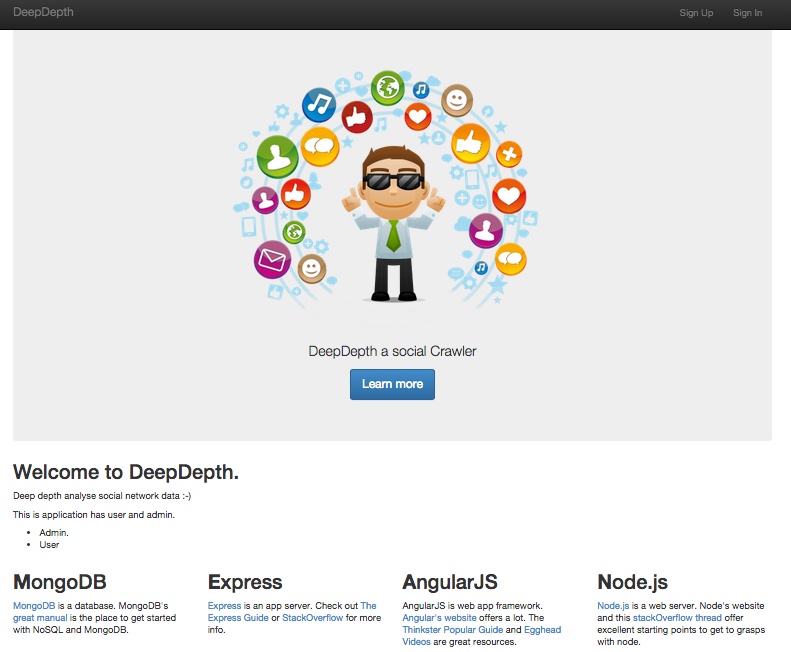
\includegraphics[scale=0.5]{dd_firstpage.png}
\end{center}
\caption{DeepDepth Home Page}
\label{fig:dd_firstpage}
\end{figure}

\subsubsection{Register and Login}

The user can register it self into DeepDepth by visiting sign up page. Figure \ref{fig:dd_register} shows that a user can sign up using his social accounts such as Facebook and Twitter or create a new Login in DeepDepth. Users are able to link their accounts to their social network accounts later in their profile settings.

\begin{figure}[H!]
\begin{center}
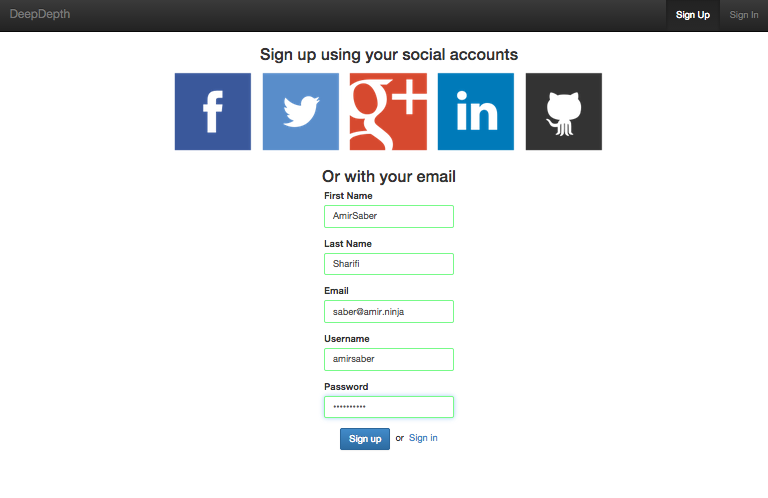
\includegraphics[scale=0.5]{dd_register.png}
\end{center}
\caption{DeepDepth Sign Up}
\label{fig:dd_register}
\end{figure}

After Registring into system users are able to login into system. Figure \ref{fig:dd_login} shows the Sign in page.

\begin{figure}[H!]
\begin{center}
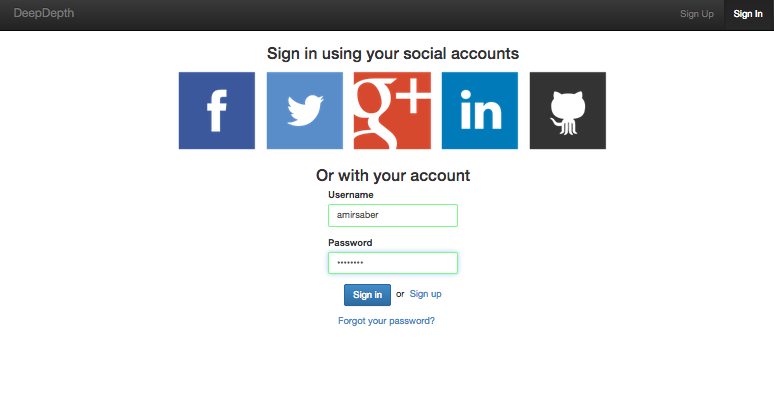
\includegraphics[scale=0.5]{dd_login.png}
\end{center}
\caption{DeepDepth Sign in}
\label{fig:dd_login}
\end{figure}

\subsubsection{Main Menu}

After signing into DeepDepth, based on the user role in system, they will see different menu items. Considering an admin user loging into system figure \ref{fig:dd_afterlogin} shows the availbale menu item for admins.

\begin{figure}[H!]
\begin{center}
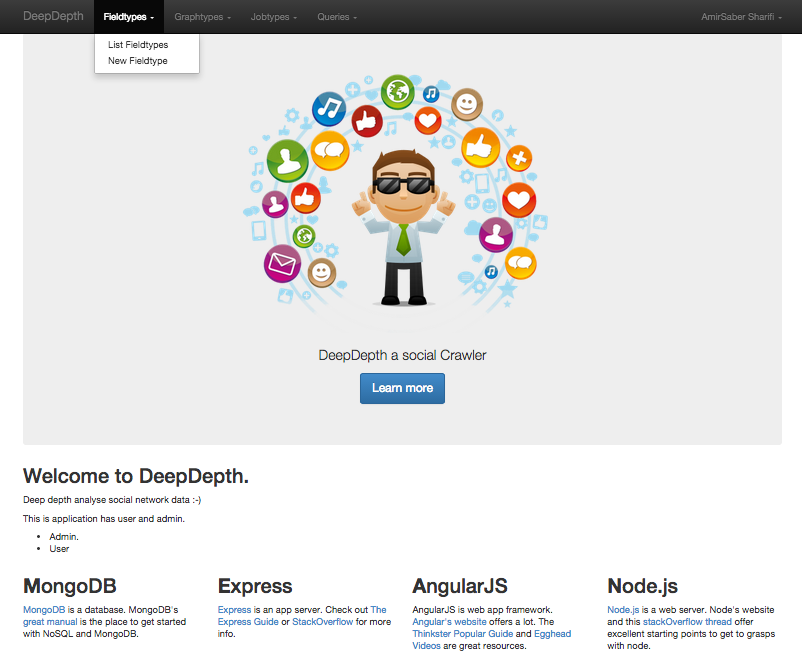
\includegraphics[scale=0.5]{dd_afterlogin.png}
\end{center}
\caption{DeepDepth Admin Menu}
\label{fig:dd_afterlogin}
\end{figure}

Each model in application has two menu items. Listing model items and creating a new item. By hovering mouse on each menu item, sub menu items can be seen. As an example considering Field types, by clicking on 'List Fieldtypes', list of created Fieldtypes will be shown. Figure \ref{fig:dd_listfieldtype} and figure \ref{fig:dd_newfieldtype} shows listing and creating interface for Fieldtypes.


\begin{figure}[H!]
\begin{center}
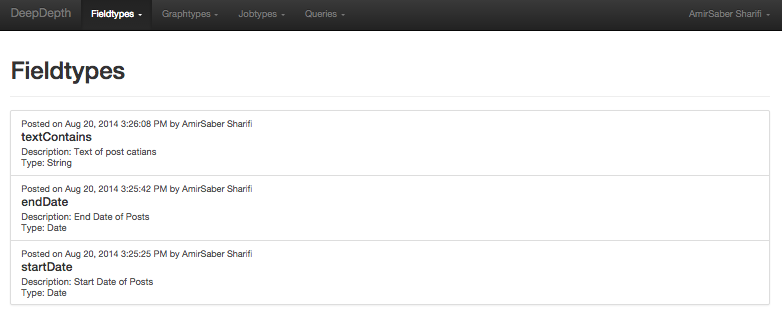
\includegraphics[scale=0.5]{dd_listfieldtypes.png}
\end{center}
\caption{DeepDepth List Field type}
\label{fig:dd_listfieldtypes}
\end{figure}

\begin{figure}[H!]
\begin{center}
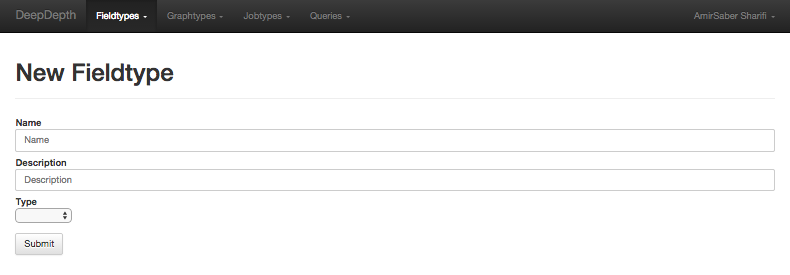
\includegraphics[scale=0.5]{dd_newfieldtype.png}
\end{center}
\caption{DeepDepth New Field type}
\label{fig:dd_newfieldtype}
\end{figure}

By clickin on each item in listing, more details will be shown. Also editing and deleting each item is availble while viewing the item. Figure \ref{fig:dd_viewfieldtype} and \ref{fig:dd_editfieldtype} show the interface for viewing and editing a FieldType. As it can bee seen, in viewing a Fieldtype two buttons are available to edit or delete that item.

\begin{figure}[H!]
\begin{center}
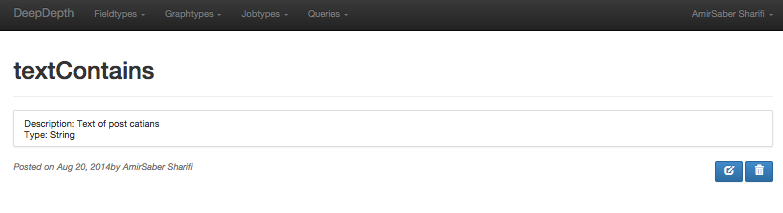
\includegraphics[scale=0.5]{dd_viewfieldtype.png}
\end{center}
\caption{DeepDepth View Field type}
\label{fig:dd_viewfieldtype}
\end{figure}

\begin{figure}[H!]
\begin{center}
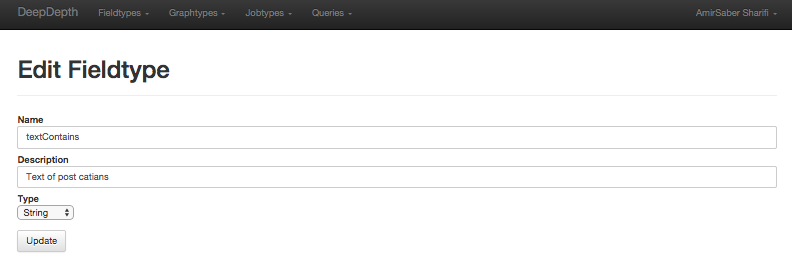
\includegraphics[scale=0.5]{dd_editfieldtype.png}
\end{center}
\caption{DeepDepth Edit Field type}
\label{fig:dd_editfieldtype}
\end{figure}

\subsubsection{Query}

Query menu is the menu which is shared between admins and users. To submit a new Query a user should login to DeepDepth and go to New Query interface by choosing it from menu Items. Then a unique name for the query should be chosen. Another required field is the Jobtype. Based on the availble Jobtypes and users requirements, Jobtype should be chosen. Afterwards a list of required Fields for that Jobtype will be shown that user should fill them to be able to submit the query. Figure \ref{fig:dd_editcreatequery} shows a query getting created. As it can bee seen in the figure, selected Jobtype is Twitter over Time and required field are filled using Ebola keyword and a time frame.

\begin{figure}[H!]
\begin{center}
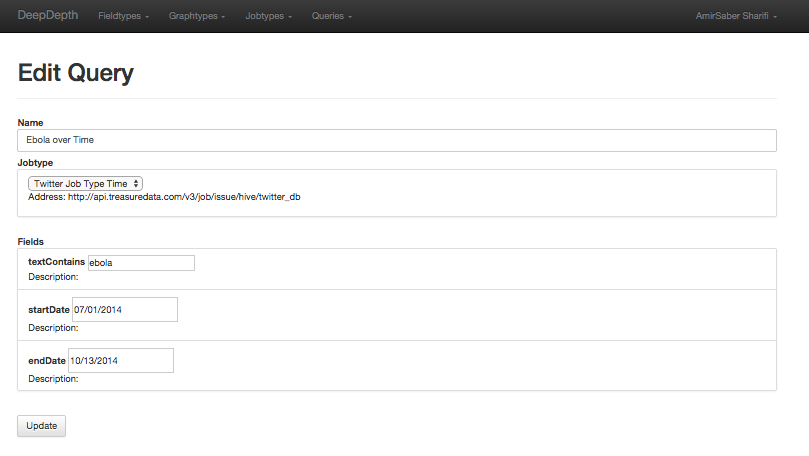
\includegraphics[scale=0.5]{dd_editcreatequery.png}
\end{center}
\caption{DeepDepth Create Query}
\label{fig:dd_editcreatequery}
\end{figure}

After submiting the query user should wait for the data to get collected from Social network database. By visiting the created query page status of the query can be checked. When the required processes are done the status will be changed to success and user can choose from the Graphtypes, the graph that is desired to view. Figure \ref{fig:dd_viewquery} shows one Graphtype for the Ebola query. It shows states of U.S. which are talking about Ebola over time and by clicking on the play button it will go through days and shows how it changes over time.

\begin{figure}[H!]
\begin{center}
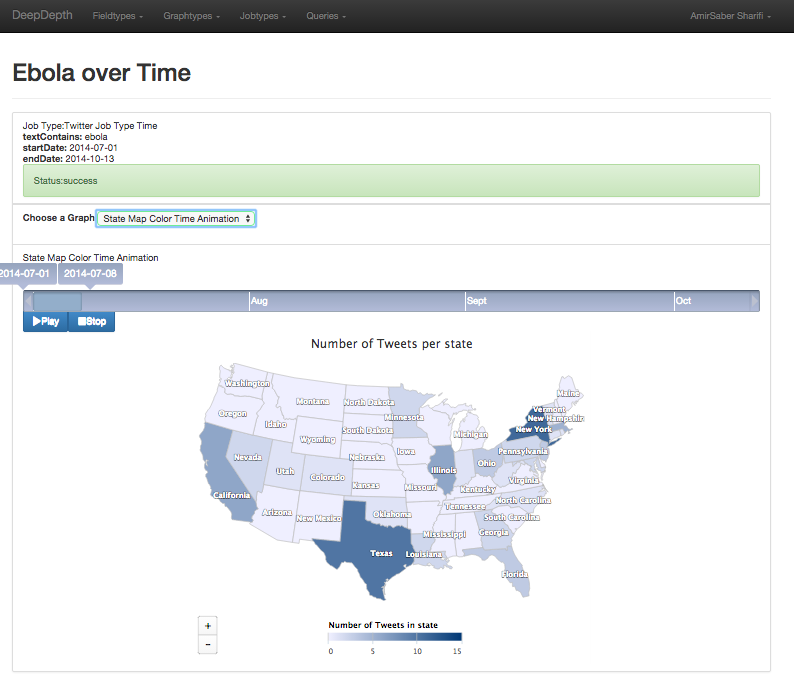
\includegraphics[scale=0.5]{dd_viewquery.png}
\end{center}
\caption{DeepDepth View Query}
\label{fig:dd_viewquery}
\end{figure}


\chapter{Summary and Future Works}

\memo{WY: This part is definitely needed. It basically summarizes what your system is about, why you think it is cool, and you can add future work here. Also, List of Figures is usually before Chapter 1 right in front of the document.

\begin{itemize}
\item Talking about summary of project and it's achievements(I am not sure if this part is needed or what should I put in here.) 
\end{itemize}

\begin{itemize}
\item How this projects can be improved in future
\item nice to have features
\end{itemize}
}

DeepDepth is a platform that helps users to analyze social networks and see graphs and analysis based on their need. On the other hand it provide the required infrastructure to developers and admins to add more features and data sources into DeepDepth. The first version of DeepDepth provides Twitter U.S. tweets as its datasource and two Jobtypes as example. Because of having the required infrastructure admins and developers can add more datasources, Jobtypes and Graphs into system.

In future, DeepDepth can be improved by getting connected to realtime data analytic systems such as Apache Storm. So users will be able to get analysis without waiting for the MapReduce job to be finished.

Another feature that can be added in next releases is that to enable users to ask admin for their desired Jobtype and Graphs. So admins will be notified on users needs and create them. Being able to share results on Social Networks and downloading Graphs for future use is another nice to have feauture in future of DeepDepth.

\begin{thebibliography}{9}

\bibitem{stankath}
	Social Network Analysis Methods and Applications, Stanley Wasserman, University of Illinois, Katherine Faust, University of South Carolina, November 1994
    
\bibitem{pescosolido}
	Pescosolido, B. 1991. "The Sociology of the Professions and the Profession of Sociology: Professional
Responsibility, Teaching, and Graduate Training." Teaching Sociology 19:351-361 (special issue on the
state of graduate education).

\bibitem{socialnetworkdef}
	BERNICE A. PESCOSOLIDO
    \url{http://www.uk.sagepub.com/leonguerrero4e/study/materials/reference/05434_socnet.pdf}
    \emph{THE SOCIOLOGY OF SOCIAL NETWORKS}  
    
\bibitem{socialwebw3}
  Halpin, Harry; Tuffield, Mischa.
  \emph{"A Standards-based, Open and Privacy-aware Social Web"}
  W3C Social Web Incubator Group Report 6th December 2010 Report. W3C Incubator Group Report. Retrieved 6/8/2011
    
\bibitem{twitterstat}
	\url{http://www.internetlivestats.com/twitter-statistics/}
    
\bibitem{twittercompany}
	\url{https://about.twitter.com/company}
    
\bibitem{orgnet}
	\url{http://www.orgnet.com/sna.html}
    
\bibitem{twazzup}
	\url{http://www.twazzup.com/}

\bibitem{twitscoop}
	\url{http://twitscoop.com/}
    
\bibitem{tweetpsych}
	\url{http://tweetpsych.com/}
    
\bibitem{tweeps}
	\url{http://www.tweeps.com/}
    
\bibitem{twitonomy}
	\url{http://www.twitonomy.com/}
    
\bibitem{twitterfirehose}
	\url{http://www.brightplanet.com/2013/06/twitter-firehose-vs-twitter-api-whats-the-difference-and-why-should-you-care/}

\bibitem{herokuadd}
	\url{https://www.heroku.com/}
    
\bibitem{treasuredataadd}
	\url{http://www.treasuredata.com/}

\bibitem{apachestormadd}
	\url{https://storm.apache.org/}
    
\bibitem{d3jsadd}
	\url{http://d3js.org/}
    

\end{thebibliography}

\end{document}
